\subsection{Using external Maps Services}
In order to compute, as well as possible, the user's calendar, the \emph{Travlendar+} service needs to know more information about the status of interested roads, the traffic information about the city and other useful information concerning the user's trip.
To reach this goal the \emph{Travlendar+} System needs to interact with an external maps service, retrieving these kind of information.

\begin{table}[H]
	\centering
    
    \begin{tabular}{|p{3.5cm}|p{10.3cm}|}
    
    \hline
    \textbf{\large{Actors}}  			& \tabitem External Maps Service\\
    
    \hline
    \textbf{\large{Goals}} 				& \ref{goal:task}; \ref{goal:reachability}; \ref{goal:timeslot}; \ref{goal:travel}; \ref{goal:piotti}\\
    
    \hline
    \textbf{\large{Enter Condition}}	& The \emph{Travlendar+} service is computing the user's calendar, so it needs to know more information about the user's trip\\
    
    \hline
    \textbf{\large{Events Flow}}		& \begin{enumerate}[leftmargin=0.5cm]
                                          	\item The \emph{Travlendar+} system asks the maps information to the \emph{External Maps} service through APIs
                                          	\item The \emph{External Maps} service sends back the maps information
                                          	\item The \emph{Travlendar+} now asks to the \emph{External Maps} service to compute a trip
                                          	\item The \emph{External Maps} service finally sends back the road trip just computed and more useful information about that journey
                                          \end{enumerate}
    										\\
    \hline
    \textbf{\large{Exit Condition}} 	& The \emph{Travlendar+} service knows all the information it needs in order to schedule as well as possible the user's calendar\\
    
    \hline
    \textbf{\large{Exception}} 			& It may be happened that the \emph{External Maps} is unavailable for some reasons, in this case the \emph{Travlendar+} system cannot compute the user's calendar, and our system tries to schedule it later with another request to the maps service\\
    
    \hline
    
    
    \end{tabular}
	
\end{table}

\begin{figure}[H]
\centering
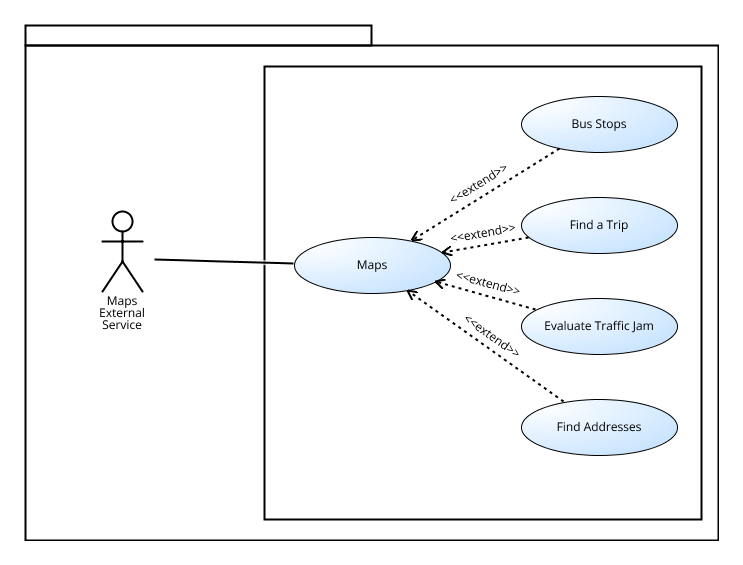
\includegraphics[scale=0.5]{Pictures/UseCaseDiagram/Google.png}
\caption{UML Use Case Diagram for the information requests about the maps}
\end{figure}